\chapter{Background \& Objectives}

%The aim of this project is to implement a UNIX command line shell that conforms to the POSIX shell standard\cite{POSIX-SHELL-STANDARD}.

%A command line shell is the minimal interface between users and the operating system kernel and allows users to work with a relatively simple read-eval-print loop.

%This section should discuss your preparation for the project, including background reading, your analysis of the problem and the process or method you have followed to help structure your work.  It is likely that you will reuse part of your outline project specification, but at this point in the project you should have more to talk about. 

%\textbf{Note}: 

%\begin{itemize}
%   \item All of the sections and text in this example are for illustration purposes. The main Chapters are a good starting point, but the content and actual sections that you include are likely to be different.
%   \item Look at the document on the Structure of the Final Report for additional guidance. 
%\end {itemize}

This Chapter provides some background information concerning the project. The first section explains the concepts and importance of a command line shell.
The second the problems that are apparent in those that are currently available.
The third 


\section{Background}

\section{Motivations}
A shell is the minimal interface between the user and the operating system kernel allowing users to directly execute programs, interact with files and devices (which can provide network access, e.g /dev/tcp/host/port) as well as providing a turing complete environment to perform interactive or automated tasks.
All linux distributions right down to the very smallest\cite{ALPINE-LINUX} include a shell and until recently many used sysVinit scripts to boot the system.
Shells have been ingrained into everyday computer science since the first generation where developed at Bell Labs (See figure~\ref{fig:shell-history}).
They have also been very influential in the design of scripting languages such as Perl and PHP. 
I began using bash once I switched my operating system to Linux in 2009 and have become a fan of it's terse syntax and quirks especially for codegolf\cite{CODE-GOLF}. %XXX

During my year in industry the ShellShock\cite{SHELLSHOCK-CVE,SHELLSHOCK-LWN,SHELLSHOCK-SYMANTEC} vulnerability was announced which drew my attention to the underlying technology.
I started examining the source code for bash once patches for shellshock and the subsequently discovered vulnerabilities were released.
The first thing I noticed was the huge amount of code that it consisted of (See table~\ref{tab:bash-loc}) and the low numbers of contributors.
While the OpenSSL codebase was in a worse state when the Heartbleed vulnerability broke earlier in the year that got two highly publicized forks attempting to modernize it (BoringSSL by Google\cite{BORINGSSL} and LibreSSL by The OpenBSD Foundation\cite{LIBRESSL}).
When nobody appeared to be attempting anything similar with bash I considered trying it myself.

A presentation on handwritten lexers\cite{PIKE-LEXING-VIDEO} given by Rob Pike, one of the creators of GoLang, intrigued me as everything seemed so simple and easy to follow. 
I had always assumed that implementing any language would have been extremely difficult as I'd only come across codebases in C that made heavy use of code generation.
Another presentation, given by Stephen Bourne, on the design of the original shell\cite{DESIGN-OF-SH-VIDEO} made it clear that it was originally designed without the use of such tools.

Along with the book, Apprenticeship Patterns\cite{APPRENTICESHIP-PATTERNS} and the blog post, What Every CompSci Graduate Should Know\cite{EVERY-COMPSCI-GRAD}, these videos made implementing a shell seem like the type of thing that would push me to learn.

\begin{table}[hp]
\centering
\caption{Lines of code in bash's latest release (4.4-rc1)}
\label{tab:bash-loc}
\begin{tabular}{@{}lrrrr@{}}
\toprule
Language           & files & blank & comment & code   \\ \midrule
C                  & 252   & 20090 & 19392   & 102608 \\
HTML               & 3     & 3762  & 39      & 25942  \\
Bourne Shell       & 36    & 3330  & 3459    & 19857  \\
Teamcenter def     & 44    & 2567  & 1491    & 13014  \\
C/C++ Header       & 111   & 2719  & 3438    & 7286   \\
yacc               & 2     & 800   & 885     & 5096   \\
m4                 & 4     & 465   & 438     & 4656   \\
Perl               & 2     & 535   & 834     & 4229   \\
Bourne Again Shell & 24    & 196   & 249     & 786    \\
make               & 3     & 48    & 36      & 110    \\
Assembly           & 2     & 11    & 20      & 48     \\
awk                & 1     & 8     & 15      & 24     \\
sed                & 2     & 0     & 0       & 16     \\ \midrule
SUM:               & 486   & 34531 & 30296   & 183672 \\ \bottomrule
\end{tabular}
\end{table}

\begin{figure}[hp]
    \centering
    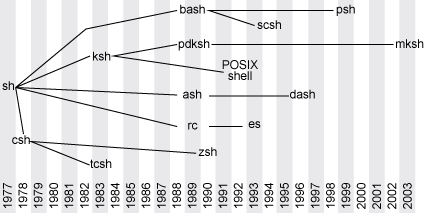
\includegraphics[width=0.8\textwidth]{xyz.png}
    \caption[Lineage of the main shells]{Lineage of the main shells\cite{SHELL-HISTORY}. Features where also incorporated across branches in many cases.}
    \label{fig:shell-history}
\end{figure}

\section{Preparation}
There are two families of shells, those descended from sh and csh, (See figure~\ref{fig:shell-history}), known as traditional shells and the so called exotic shells that have a syntax largely incompatible with other shells. Fish\cite{FISH}, es\cite{ES-SHELL} and oh\cite{OH-SHELL} are examples of exotic shells.

To prepare for this project I started examining the source code for some of the modern traditional shells, including bash, dash and zsh.


dash is a POSIX compliant shell which lacks many features useful in an interactive context.
Bash adds things such as history control, line editing and arrays but also has a compatibility mode for POSIX scripts.
Zsh has many extra features but also has emulation modes for its major rivals though they are not 100\% compatible. 

To learn about compiler construction and language design I started studying from some of the courses available online that don't advocate using auto generation tools\cite{COMPILERS-COURSE,CRENSHAW}.
I also scanned through a book on lex\&yacc as both the are used in the bash source code and I wanted to be able to understand their use.

% ---------------------
and reading books\cite{LEX-AND-YACC} and articles\cite{BUILD-INTERP,GOPHER-LEXING-BLOG} related to language design and compiler/interpretor construction. 


% ---------------------

% What was your background preparation for the project? What similar systems did you assess? What was your motivation and interest in this project? 

\section{Analysis} %========================================================

My original intention was to create a drop in replacement for bash but after examination of the source code for various shells it became clear that this was too ambitious.
The order of magnitude difference in lines of code between dash (Table~\ref{tab:dash-loc}) and bash (Table~\ref{tab:bash-loc}) suggests that the extra features present would add a huge amount of time to development and it would have been impossible to complete in the given time frame.
Despite this I want to develop the code so that after submission I can continue working on it to eventually reach my initial goal.

\begin{table}[hp]
\centering
\caption{Lines of code in dash's latest release (0.5.8)}
\label{tab:dash-loc}
\begin{tabular}{@{}lrrrr@{}}
\toprule
Language       & files & blank & comment & code  \\ \midrule
C              & 36    & 2120  & 2382    & 13153 \\
C/C++ Header   & 33    & 244   & 1049    & 1193  \\
make           & 2     & 100   & 38      & 655   \\
Bourne Shell   & 2     & 18    & 76      & 116   \\
Python         & 1     & 24    & 46      & 75    \\
Teamcenter def & 1     & 8     & 10      & 34    \\ \midrule
SUM:           & 75    & 2514  & 3601    & 15226 \\ \bottomrule
\end{tabular}
\end{table}

With that in mind I set out the high level objectives for the project.

\begin{itemize*}
    \item Create a POSIX\cite{POSIX-SHELL-STANDARD} compliant shell.
    \item Produce maintainable and easy to extend code.
    \item Provide a meaningful test suite consisting of both unit and integration tests.
    \item Become a more experienced Golang developer with a good portfolio piece.
\end{itemize*}

Some of these goals are vague and subjective but most importantly they don't make good assessment criteria.
To come up with them we need to look at a combination of what users expect from a shell and what the POSIX specification requires the shell to do.

The man page for the rc shell begins with:
\begin{lstlisting}
All of the following behave as expected:

date
cat /lib/news/build
who >user.names
who >>user.names
wc <file
echo [a-f]*.c
who | wc
who; date
vc *.c &
mk && v.out /*/bin/fb/*
rm -r junk || echo rm failed!
\end{lstlisting}

While this may not look like much it showcases a good portion of the features that most user's need in their shell:
\begin{itemize*}
    \item Command execution with optional arguments.
    \item IO redirection to and from files.
    \item Filename and path globbing.
    \item Pipelining (IO redirections to concurrently running commands).
    \item Command chaining.
    \item Asynchronous commands.
    \item Conditional execution.
\end{itemize*}
The fact that these have been explicitly pointed out to work shows that these are some of the most important features.

Despite this I have decided to give development of IO redirection a low priority as it can be emulated through the use of pipes and utilities. \\
For example; output to a file \verb!foo | tee [--append] output_file! \\
and for input to a command \verb!cat input_file | foo!.\\
While these do not cover the full range of redirections, such as redirecting standard error, they will suffice to cover most situations and mean that development can be focused in other areas.

Along with these features the shell also needs:
\begin{itemize*}
    \item Variables, variable substitution and scoped variables
    \item Shell functions.
    \item Command substitution / Subshells.
    \item Arithmetic substitution.
    \item Shebang support (e.g \#!/bin/foo)
    \item Control structure (if, while, until, for, case, functions)
\end{itemize*}

These features are gathered from the POSIX specification.

This leaves out an important aspect of most shells, interactivity.
I decided that sticking to a shell that runs shell scripts well would be preferable to having one with readline support but that didn't work properly. There is a Go implementation that offers the required functionality\cite{GO-READLINE} so this would be a good extension if time allows.

My main analysis was based on the dash shell\cite{DASH} as it conforms to the POSIX shell standard\cite{POSIX-SHELL-STANDARD} while still having a reasonably small code base.
I also used the ash shell implementation included in busybox\cite{BUSYBOX} because of it's similarities.

The first thing you notice is that everything is built around three components, the Parser, the Lexer and a function called evaltree.
The lexer takes the raw string representation of the program and splits it into tokens.
These are feed, along with their values when appropriate, to the parser.
The parser intelligently groups these tokens into nodes representing high level structure inside the program.
This structure is known as an Abstract Syntax Tree(AST) and items in the tree are referred to as nodes.
The tree is then passed to the evaltree function which performs all of the actions contained within it.
It would also be possible to do away with the abstract syntax tree and interpret the code as it is parsed.

I decided against this for multiple reasons.
\begin{enumerate*}
	\item Separating the concerns of running a certain command from the parser means that a parse error will never leave execution in some undefined state.
	\item The tight coupling of the lexer, parser and evaluation would make it difficult to extend code in the future.
	\item All the texts I read encourage creating an AST for any future translations or optimizations. If at some point I decide I wanted to compile shell scripts to native binaries it would be impossible without one.
\end{enumerate*}

While these are the most important parts of the system as a whole I decided that starting with the arithmetic environment ( \$(( )) ) would be a good idea.
This construct is sufficiently complex that it requires it own lexer and parser pair to keep the overall structure of the code simple but it is still just a glorified calculator.
Creating the lexer \& parser for this relatively simple language would give me experience working with them before I attempted to move onto the more complex main parser.


% ---------------------
These three components are some of the most important aspects of the code but they still will not operate correctly without other pieces of code being in place, such as the variable assignment and retrieval routines.

While this lexer and parser pair is quite complicated it should be possible to build so a single feature at a time is added to it.

Something that is notable is the use of global variables to hold parser and lexer state.

The first thing you notice about each shell is the general lack of comments, while the figures in table~\ref{tab:dash-loc} seem to show a good ratio of code:comments most of these are in fact repeated license headers in files.
This means it is both confusing and discouraging for newcomers to the codebase. 



Zmalloc

Linked Lists -> hash tables

Using the right data type where needed (nlflag should be a descriptive ENUM not int / tokpushback should be bool not int that is incr'ed, Be a function like hasNextToken)

Misleading names (CHKNL, why does it have to be short + it isnt checking newlines it is ingoring them)
% ---------------------

%Taking into account the problem and what you learned from the background work, what was your analysis of the problem? How did your analysis help to decompose the problem into the main tasks that you would undertake? Were there alternative approaches? Why did you choose one approach compared to the alternatives? 


%There should be a clear statement of the objectives of the work, which you will evaluate at the end of the work. 

%In most cases, the agreed objectives or requirements will be the result of a compromise between what would ideally have been produced and what was felt to be possible in the time available. A discussion of the process of arriving at the final list is usually appropriate.

\section{Process}
%You need to describe briefly the life cycle model or research method that you used. You do not need to write about all of the different process models that you are aware of. Focus on the process model that you have used. It is possible that you needed to adapt an existing process model to suit your project; clearly identify what you used and how you adapted it for your needs.

The process that I followed was a combination of Feature Driven Development (FDD) and Test Driven Development (TDD).
A combination approach was used since at the beginning of the project it was impossible to showcase features in a meaningful way.
TDD was used during the first few weeks as it allowed me to show progress, prevent regressions and explicitly document the abilities of the code I was producing.
I switched to using the FDD approach once the code had become more stable and I had gained more experience and understanding of the complexities of the project.

This process suited the project very well as I was a single person team with only one meeting a week with my project supervisor.
Being able to announce that a certain list of the features would be completed over the next week really drove me to work on them so I could prove I was making progress at each subsequent meeting.
Having a design that consisted of these feature sets and individual features was also hugely helpful as time progressed and we realised that the scope of the project would have to be reduced.

FDD also lent itself well to this project as the overall model and feature list was provided to me in the form of the specification.
However the feature descriptions in the specification go into a large amount of extraneous implementation detail.
This detail could easily be ignored for the high level design and left to be incorporated into the feature design step.
Using the spec in this way allowed me to jump straight to implementing features once enough of the codebase was there to support them.

While I supplanted TDD with the more complete process of FDD they are complimentary techniques and often used together.
One of the steps of the feature build is code inspections and how this is done is decided on by the Team leader, called a Chief Programmer in FDD terminology.
It will often a combination of code review and testing, which in many modern development teams these tests is likely to be performed in a TDD manor.
I continued with unit tests and started adding integration tests once I switched process.
The confidence these tests gave allowed me to easily add and refactor features while ensuring that everything still worked as intended.  

One of the things I liked best about using this process was the constant feedback it gave me on the progression of the project.
If I became stuck on a certain feature I could always switch working branches and attempt to complete a smaller feature giving me time to think out the problems I had encountered with the other one.
Upon completion of a feature I always received a morale boost which really helped focus me on achieving the next goal in my list\cite{GETTING-REAL}.

During the development of my project, excluding the Easter holidays, I programmed with a friend who was working on their own project, which allowed us to keep each other motivated.
We often used each other for so called rubber duck debugging\cite{RUBBER-DUCK-DEBUG} which was very helpful. 
Comments made to each other on design and features usually provided insight into something we otherwise wouldn't have considered.

















